\subsection{Fen\'omenos que afectan al comportamiento de los circuitos (limitaciones)} %VER SI DEJAR PARA C/CASO O AL FINAL, for BOTH, o al ppio introductoriamente
	\subsubsection{Efecto de slew rate (SR)}
	El Slew Rate es un fen\'omeno que se produce a la salida de un amplificador operacional, 
	por el cual la se\~nal de salida se ve alterada respecto de la se\~nal de entrada. 
	Esta alteraci\'on se produce en aquellos segmentos temporales donde la derivada de 
	la se\~nal de salida $te\'orica$ (es decir, la que seg\'un el modelo se deber\'ia observar 
	a la salida) supera un determinado valor, especificado por el fabricante del circuito 
	integrado en su respectiva hoja de datos. En esos casos, la pendiente de la se\~nal se ver\'a 
	limitada a la indicada por este coeficiente. A continuaci\'on se muestra la ecuai\'on que define
	al slew rate (SR):

	\begin{equation}
		SR = m\'ax\bigg\{\frac{ dV_{out}}{dt}\bigg\}
		\label{srr}
	\end{equation}

	Para el caso del circuito integrado utilizado (LM324 de Texas Instruments) 
	el valor del slew rate es de $0.5 \frac{V}{\mu s}$. Esto fue obtenido a partir
	del gr\'afico \ref{srdatasheet} presentado por el fabricante. 

	\begin{figure}[H] %!ht
		\centering
		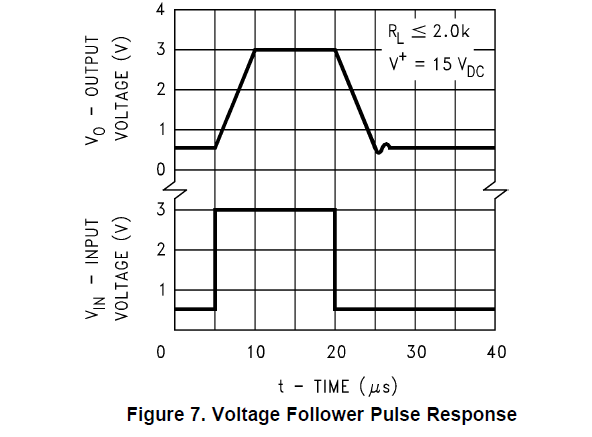
\includegraphics[width=10cm,height=10cm,keepaspectratio]{../EJ1/00GRAFICOS/SRdatasheet.png}
		\caption{Gr\'afico de la hoja de datos de la que se obtuvo el valor del slew rate.}
		\label{srdatasheet}
	\end{figure}

	El valor sale de calcular la pendiente de la tensi\'on de salida como respuesta a la se\~nal cuadrada de entrada, a partir del cociente entre $\Delta V$ y $\delta t$ como se ve en la figura \ref{srt}.

	\begin{figure}[H] %!ht
		\centering
		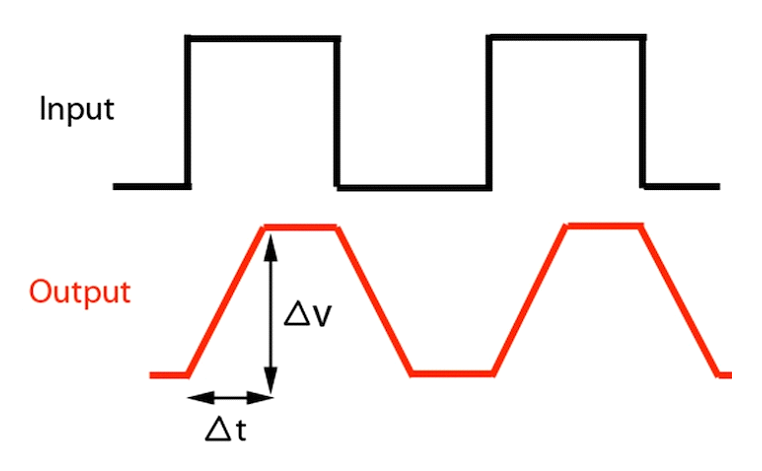
\includegraphics[width=10cm,height=10cm,keepaspectratio]{../EJ1/00GRAFICOS/srt.png}
		\caption{Detalles del gr\'afico para el c\'alculo del slew rate.}
		\label{srt}
	\end{figure}

	A continuaci\'on se presenta una imagen del osciloscopio mostrando el efecto que fue observando en la pr\'actica.

	\begin{figure}[H] %!ht
		\centering
		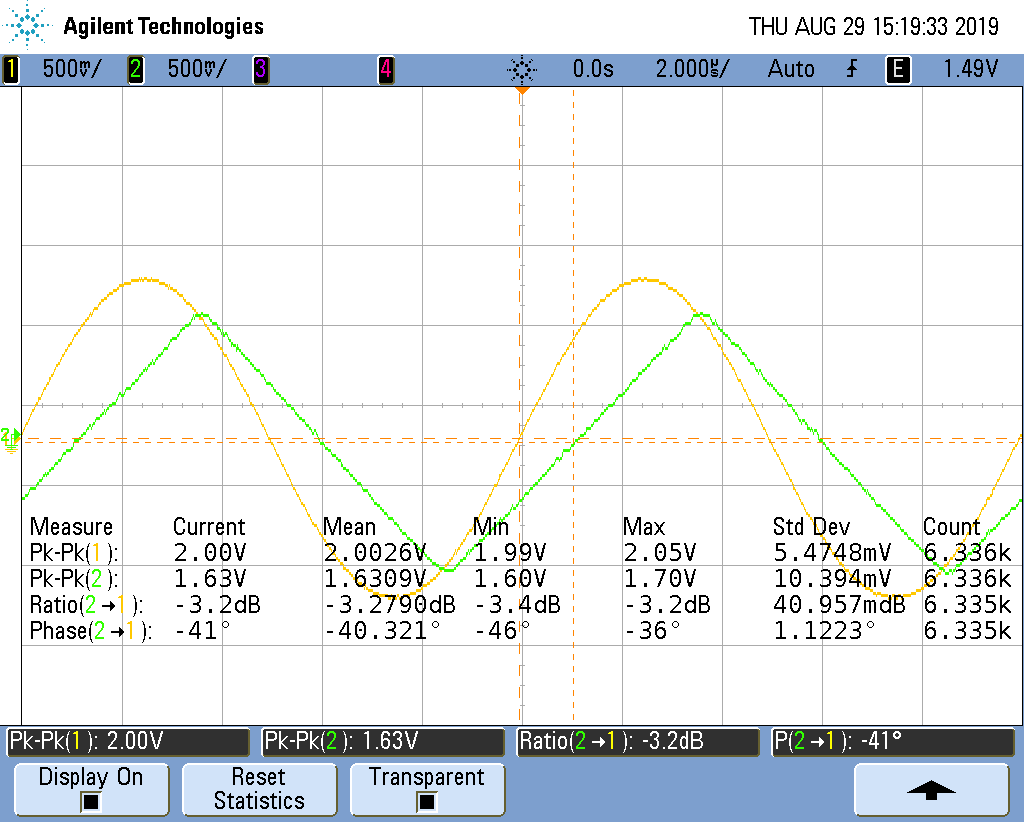
\includegraphics[width=10cm,height=10cm,keepaspectratio]{../EJ1/00GRAFICOS/srm.png}
		\caption{Efecto de slew rate observado en el osciloscopio.}
		\label{srm}
	\end{figure}

	Se midi\'o el slew rate alimentando uno de los circuitos con una se\~nal senoidal de 3Vpp y 800KHz;
	ya que en esas condiciones a la salida se pod\'ia observar dicho efecto. Se colocaron los cursores en 
	una posici\'on que permitiera calcular la pendiente y se obtuvo:
	\begin{equation}
		\begin{cases}
			\Delta X = 466 ns \\
			\Delta Y = 246 mV
		\end{cases}
		\label{srmedicion}
	\end{equation}

	y por lo tanto, $SR = 0,526 \frac{V}{\mu s}$, lo cual coincide mucho con el valor de la hoja de datos.
	

	Esta distorsión en la se\~nal obliga a tener ciertas consideraciones en las mediciones. 
	Por ejemplo, en el caso de la medici\'on de respuesta en frecuencia de los circuitos, 
	en donde es de vital importancia conocer el valor pico a pico de la se\~nal de salida, 
	se debe cuidar que el producto de la frecuencia de excitaci\'on y la amplitud de salida no
	 exceda al coeficiente de slew rate, como mínimo. Caso contrario la señal senoidal tenderá 
	 a ser triangular, con lo cual las mediciones no serán útiles. Como consecuencia de esto, 
	 a medida que se aumenta la frecuencia de la entrada se debe moderar la amplitud de esta 
	 señal, para evitar la aparición de slew rate en la salida.

	 Según se pudo investigar, el origen de esta limitación se encuentra en el agregado de un 
	 capacitor de compensación en el circuito interno del operacional, el cual se utiliza 
	 para modificar la respuesta en frecuencia del mismo amplificador. Por otro lado, en 
	 la práctica se desprecie este efecto en la mayoría de los casos, dado el alto coeficiente 
	 de slew rate que poseen algunos circuitos integrados en la actualidad. 



	\subsubsection{Distorsi\'on de cruce por cero (Cross-Over Distortion)}
	Otro fenómeno para tener en cuenta al momento de efectuar mediciones es el
	 denominado “crossover distortion”. Este efecto se hace presente cuando la tensión 
	 de entradas se aproxima a cero, u oscila en un rango aproximado de -0.7V a 0.7V.
	  Estas últimas dos tensiones son justamente aquellas que accionan un diodo de silicio, 
	  y análogamente describen las tensiones base-emisor de un transistor BJT.
Podemos modelar a la salida de un amplificador operacional como dos transistores 
(uno NPN y otro PNP) dispuestos como se muestra en la siguiente figura \ref{cross}. Esto es tenido en cuenta 
ya que internamente el amplificador operacional tiene transistores que generan este comportamiento.

\begin{figure}[H] %!ht
	\centering
	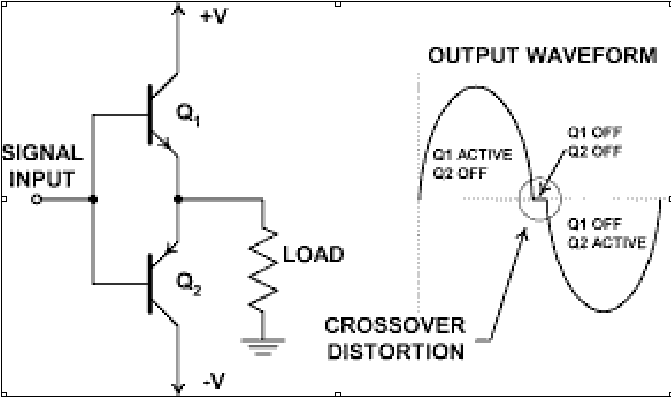
\includegraphics[width=10cm,height=10cm,keepaspectratio]{../EJ1/00GRAFICOS/cross.png}
	\caption{Efecto de crossover distortion.}
	\label{cross}
\end{figure}

Cuando la tensi\'on de input se acerca a los rangos antes mencionados, 
un transistor se pone en modo de corte y el otro en modo saturaci\'on. 
En esta conmutaci\'on entre transistores se produce un efecto alineal, 
dada la alinealidad de la curva característica de salida de un transistor. 
De esta forma, la señal de salida no $sigue$ en forma a la se\~nal de entrada, 
por lo que se produce una ruptura en el lazo de alimentación en el circuito. 
Luego, obtenemos un recorte de la señal de salida, como se muestra en la figura anterior. 
Esto nuevamente tiene impacto sobre la medici\'on de la señal, dado que esta no refleja 
el comportamiento esperado del circuito. Para compensar este efecto se encontró que es 
especialmente \'util superponer un nivel de continua sobre la señal que se inyecte al circuito. 
Esto ayuda a disminuir este efecto, en la mayor\'ia de los casos. Dicho nivel de offset en la se\~nal fue agregado de forma totalmente empírica a cada medición, en función de lo reflejado en la salida en la pantalla del osciloscopio.
A continuación se muestran ejemplos de esta distorsi\'on en las sucesivas mediciones practicadas.


	\subsubsection{Gain Bandwidth Product (GBP)}
	El gain-bandwidth product (o GBP por sus siglas) es el producto entre el ancho de banda 
	y la ganancia máxima que presenta el amplificador operacional. El ancho de banda est\'a
	definido por la frecuencia para la cual hay una ca\'ida de 3dB de la tensi\'on de salida
	respecto a la de entrada del circuito. Esto puede ser visto facilmente en la respuesta
	en frecuencia de un circuito en la ubicaci\'on del primer polo. Los amplificadores
	operacionaes tienen un polo dominante. Dado que se comportan como un pasa bajos, dicho 
	polo es aqu\'el que determina la frecuencia para la cual hay atenuaci\'on de 3dB. El polo 
	dominante depende de los componentes internos del operacional, por lo que cada amplificador
	operacional tiene un polo dominante diferente, y por lo tanto un ancho de banda distinto. Esto
	significa que seg\'un la frecuencia a la cual se desea trabajar, se deber\'a elegir un 
	amplificador operacional que defina un ancho de banda que abarque la regi\'on de frecuencias 
	requerida en el dise\~no del circuito, ya que influyer\'a en la respuesta en frecuencia
	del circuito.
	

	\subsubsection{saturación}
	Según el modelo simplificado e ideal de un amplificador operacional, lo único que rige a la señal de salida es la ganancia del componente respecto de la señal de entrada, presentando un comportamiento netamente lineal. Es decir, si tenemos una configuración de amplificador cuya ganancia es 1000, e inyectamos una señal cuyo valor pico a pico es de 1V, la salida será de igual forma a la entrada con un valor pico a pico de 1000V.
En la práctica el circuito integrado que contiene a los amplificadores operacionales está alimentado por una fuente de corriente continua constante (en este caso simétrica) que es la que entrega la potencia en el momento de amplificar una señal. Esta aproximación a la realidad supone una restricción al circuito, siendo esta que los valores máximos y mínimos de la señal de salida nunca podrán superar a los valores máximos y mínimos de alimentación (+Vcc, -Vcc), respectivamente. Como consecuencia de esto, la salida del circuito entrará en estado de “saturación” cuando la tensión de salida sobrepase los límites de la alimentación, lo que deriva en un comportamiento alineal de la salida. 

Al llevar a cabo el DC sweep del cual se habl\'o previamente, se pudo observar que no hab\'ia forma de llegar realmente a los $\pm 15V$ a la salida,
que es la tensi\'on de $V_{cc}$ con la que se alimentaba al integrado, sino que la saturaci\'on se daba cerca de los 14V. Esto se debe a que en la realidad
la saturaci\'on ocurre un poco antes debido a caracter\'isticas de c\'omo est\'a hecho internamente el integrado.
Por lo tanto, esto se puede deber a alguna ca\'ida de tensi\'on interna dentro del amplificador operacional no predicha en el modelo teórico (como por ejemplo caídas de tensión para la alimentación de los transistores que componen la lógica interna del amplificador).
\subsection{Condiciones de comportamiento lineal del circuito}

\subsubsection{An\'alisis te\'orico}

La tensión de entrada máxima del circuito está limitada principalmente 
por el slew rate slew rate y la saturaci\'on. 

\subsubsection*{Influenccia del slew rate en $V_{in_{max}}$}

Partiendo de:
\begin{equation}
\begin{cases}
	SR = m\'ax\bigg\{\frac{ dV_{out}}{dt}\bigg\} \\
	V_{in} (f, t) = V_{in_{max}} \cdot sin(2\pi f t) \\
	V_{out} (f, t) = \rvert H(f)\rvert \cdot V_{in_{max}} \cdot sin(2 \pi f t)
\end{cases}
\label{srecs}
\end{equation}
 
Siendo $SR$ el slew rate, $V_{in}$ y $V_{out}$ las se\~nales de entrada y de salida respectivamente y $\rvert H(f)\rvert = V_{out}/V_{in}$ la ganancia del circuito.


\begin{equation}
	\frac{dV_{out}}{dt} = \rvert H(f)\rvert V_{in_{max}} 2 \pi f cos(2 \pi f t)
\label{deriv}
\end{equation}

Maximizando la ecuaci\'on \ref{deriv} se obtiene que:

\begin{equation}
	SR = m\'ax\bigg\{\frac{dV_{out}}{dt}\bigg\} = \rvert H(f)\rvert 2 \pi f V_{in_{max}} 
\label{max}
\end{equation}

Despejando de la ecuaci\'on \ref{max}:

\begin{equation}
	 V_{in_{max}}  = \frac{SR}{\rvert H(f)\rvert 2\pi f}
	 \label{vinmax}
\end{equation}

El valor de SR, para el c\'alculo te\'orico, fue sacado de hojas de datos del amplificador operacional LM324 de Texas Instrument\footnote{Hoja de datos del operacional LM324: http://www.ti.com/lit/ds/symlink/lm324-n.pdf}.
Se encontr\'o que $SR = 0,5 \frac{V}{\mu s}$. Reemplazando con este valor y con los valores correspondientes de resistencias:

%%%%%%%%%%%%%%%%%%%%%%%%%%%%%%%%%%%%%%%%%%%%%%%%%%%%%%%%%%%
\subsubsection*{- Configuraci\'on inversora}

\begin{table}[h!]
	\centering
	\begin{tabular}{c c c }%
		\bfseries  & $\bm{V_{in_{max}}}$ \\ \hline
		caso 1 & $\frac{3.38 \cdot 10^{-9} \sqrt{1.87 \cdot 10^{15} f^{2} + 8.68 \cdot 10^{24}}}{f}$\\ \\
		caso 2 & $\frac{1.86 \cdot 10^{-8} \sqrt{6.17 \cdot 10^{13} f^{2} + 8.68 \cdot 10^{24}}}{f}$ \\ \\
		caso 3 & $\frac{3.38 \cdot 10^{-9} \sqrt{1.87 \cdot 10^{15} f^{2} + 8.68 \cdot 10^{26}}}{f}$ \\
		\hline
	\end{tabular}
	\caption{Circuito inversor: Tensi\'on de entrada m\'axima, limitada por slew rate.}
	\label{vin_max}
\end{table}

\begin{figure}[H] %!ht
	\centering
	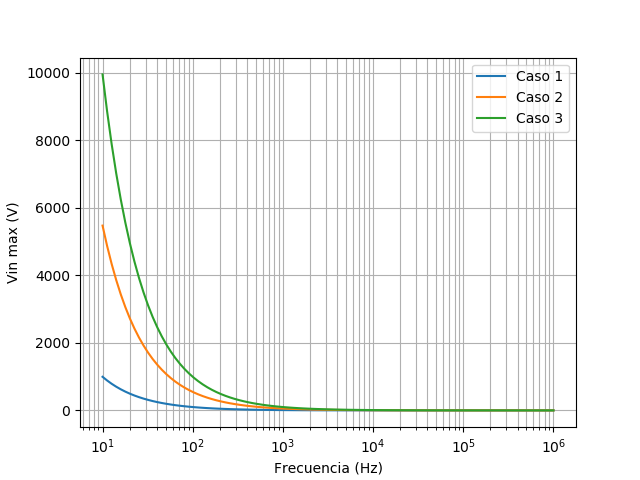
\includegraphics[width=10cm,height=10cm,keepaspectratio]{../EJ1/00GRAFICOS/teoricos/c1sr.png}
	\caption{Circuito inversor: Tensi\'on de entrada m\'axima limitada por slew rate.}
	\label{c1sr}
\end{figure}

\subsubsection*{- Configuraci\'on no inversora}

\begin{table}[h!]
	\centering
	\begin{tabular}{c c c }%
		\bfseries  & $\bm{V_{in_{max}}}$ \\ \hline
		caso 1 & $\frac{3.38 \cdot 10^{-9} \sqrt{1.87 \cdot 10^{15} f^{2} + 8.68 \cdot 10^{24}}}{f}$ \\ \\
		caso 2 & $\frac{1.86 \cdot 10^{-8} \sqrt{6.17 \cdot 10^{13}f^{2} + 8.68 \cdot 10^{24}}}{f}$ \\ \\
		caso 3 & $\frac{3.38 \cdot 10^{-9} \sqrt{1.87 \cdot 10^{15} f^{2} + 8.68 \cdot 10^{26}}}{f}$ \\
		\hline
	\end{tabular}
	\caption{Circuito no inversor: Tensi\'on de entrada m\'axima limitada por slew rate.}
	\label{vin_max}
\end{table}

\begin{figure}[H] %!ht
	\centering
	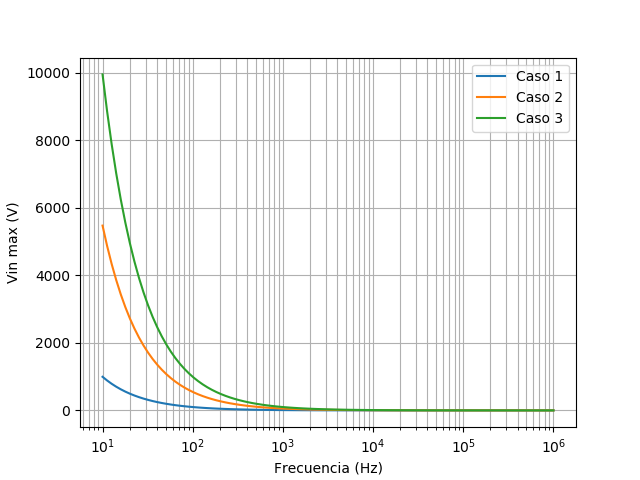
\includegraphics[width=10cm,height=10cm,keepaspectratio]{../EJ1/00GRAFICOS/teoricos/c2sr.png}
	\caption{Circuito no inversor: Tensi\'on de entrada m\'axima limitada por slew rate.}
	\label{c2sr}
\end{figure}

%%%%%%%%%%%%%%%%%%%%%%%%%%%%%%%%%%%%%%%%%%%%%%%%%%%%
\subsubsection*{Influenccia de la saturaci\'on en $V_{in_{max}}$}
La tensi\'on pico a pico m\'axima de salida del amplificador operacional es llamada 
tensi\'on de saturasi\'on $V_{sat}$. Te\'oricamente, este valor es igual a $V_{CC}$. Dado que $V_{out} = \rvert H(s) \rvert V_{in}$:

\begin{equation}
	V_{in_{max}} = \frac{V_{out_{max}}}{\rvert H(s) \rvert} = \frac{V_{sat}}{\rvert H(s) \rvert} = \frac{V_{CC}}{\rvert H(s) \rvert}
\end{equation}

Dado que en nuestro caso usamos $V_{CC} = \pm15V$, la expresi\'on que se obtiene es:

\begin{equation}
	V_{in_{max}} = \frac{15V}{\rvert H(s) \rvert} 
\end{equation}

%%%%%%%
\subsubsection*{- Configuraci\'on inversora}

\begin{table}[h!]
	\centering
	\begin{tabular}{c c c }%
		\bfseries  & $\bm{V_{in_{max}}}$ \\ \hline
		caso 1 & $5.79 \cdot 10^{-13} \sqrt{1.87 \cdot 10^{15} f^{2} + 8.68 \cdot 10^{24}}$\\
		caso 2 & $3.18 \cdot 10^{-12} \sqrt{6.17 \cdot 10^{13} f^{2} + 8.68 \cdot 10^{24}}$ \\
		caso 3 & $5.79 \cdot 10^{-13} \sqrt{1.87 \cdot 10^{15} f^{2} + 8.68 \cdot 10^{26}}$\\
		\hline
	\end{tabular}
	\caption{Circuito inversor: Tensi\'on de entrada m\'axima, limitada por saturaci\'on.}
	\label{vin_maxS}
\end{table}


\begin{figure}[H] %!ht
	\centering
	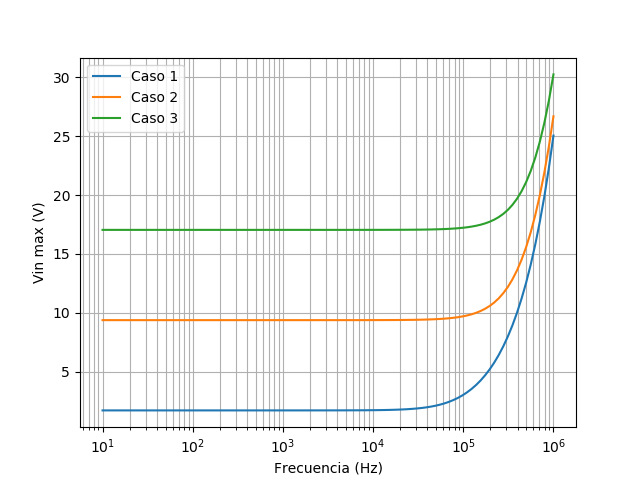
\includegraphics[width=10cm,height=10cm,keepaspectratio]{../EJ1/00GRAFICOS/teoricos/c1sat.png}
	\caption{Circuito inversor: Tensi\'on m\'axima de entrada limitada por saturaci\'on.}
	\label{c1sat}
\end{figure}

%%%%%%%%%%%
\subsubsection*{- Configuraci\'on no inversora}

\begin{table}[h!]
	\centering
	\begin{tabular}{c c c }%
		\bfseries  & $\bm{V_{in_{max}}}$ \\ \hline
		caso 1 & $ 5.79 \cdot 10^{-13} \sqrt{1.87 \cdot 10^{15} f^{2} + 8.68 \cdot 10^{24}}$\\ \\
		caso 2 & $3.18 \cdot 10^{-12} \sqrt{6.17 \cdot 10^{13} f^{2} + 8.68 \cdot 10^{24}}$ \\ \\
		caso 3 & $5.79 \cdot 10^{-13} \sqrt{1.87 \cdot 10^{15} f^{2} + 8.68 \cdot 10^{26}} $\\
		\hline
	\end{tabular}
	\caption{Circuito no inversor: Tensi\'on de entrada m\'axima, limitada por saturaci\'on.}
	\label{vin_maxS}
\end{table}

\begin{figure}[H] %!ht
	\centering
	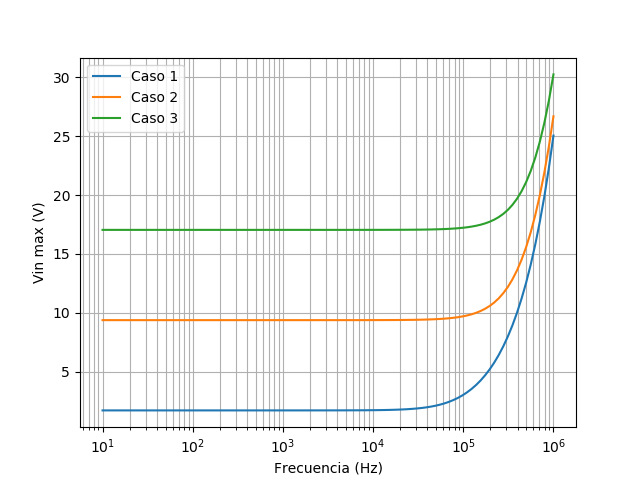
\includegraphics[width=10cm,height=10cm,keepaspectratio]{../EJ1/00GRAFICOS/teoricos/c2sat.png}
	\caption{Circuito no inversor: Tensi\'on m\'axima de entrada limitada por saturaci\'on.}
	\label{c2sat}
\end{figure}

%%%%%%%%%%%%%%%%%%%%%%%%%%%%
\subsubsection*{Combinaci\'on del efecto de slew rate y saturaci\'on sobre la tensi\'on m\'axima de entrada}

\begin{figure}[H] %!ht
	\centering
	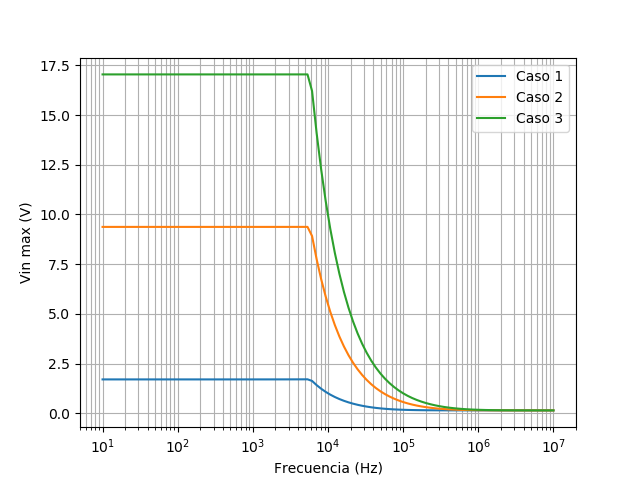
\includegraphics[width=10cm,height=10cm,keepaspectratio]{../EJ1/00GRAFICOS/teoricos/c1vimax.png}
	\caption{Circuito inversor: Tensi\'on m\'axima de entrada limitada por slew rate y saturaci\'on.}
	\label{c1vinmax}
\end{figure}

\begin{figure}[H] %!ht
	\centering
	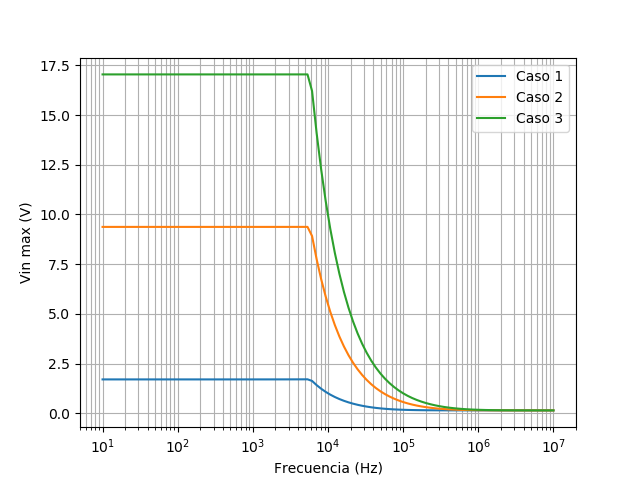
\includegraphics[width=10cm,height=10cm,keepaspectratio]{../EJ1/00GRAFICOS/teoricos/c2vimax.png}
	\caption{Circuito no inversor: Tensi\'on m\'axima de entrada limitada por slew rate y saturaci\'on.}
	\label{c2vinmax}
\end{figure}


\subsubsection{Mediciones y resultados obtenidos}
Para encontrar de forma pr\'actica la tensi\'on de entrada m\'axima, se utiliz\'o el osciloscopio en 
modo MATH, FFT, para observar la tensi\'on de entrada a partir de la cu\'al comenzaban a aparecer m\'as arm\'onicos
de lo observado a tensi\'on baja, lo cual indica que se comienza a distorsionar la se\~nal de salida. se fue subiendo la tensi\'on pico a pico de una senoidal de entrada para ver
a partir de qu\'e valor ocurr\'ia dicha distorsi\'on. Utilizando una senoidal de 100KHz, para el circuito inversor se obtuvo:

\begin{table}[h!]
	\centering
	\begin{tabular}{c c c}%
		\bfseries  & $V_{in} m\'axima$ \\ \hline
		caso 1 & $415mV$\\
		caso 2 & $270mV$ \\
		caso 3 & $285mV$ \\
		\hline
	\end{tabular}
	\caption{Tensi\'on de entrada m\'axima sin distorsi\'on a la salida.}
	\label{casos}
\end{table}

